\documentclass{standalone}
\usepackage{tikz}

\begin{document}
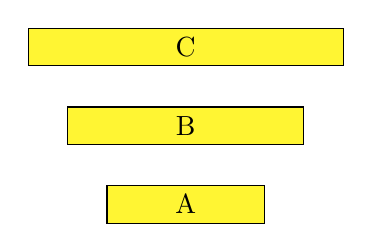
\begin{tikzpicture}[node distance=1cm]
    \node[draw, fill=yellow!80, minimum width=2cm] (A) {A};
    \node[draw, fill=yellow!80, minimum width=3cm, above of=A] (B) {B};
    \node[draw, fill=yellow!80, minimum width=4cm, above of=B] (C) {C};
\end{tikzpicture}
\end{document}